%% The first command in your LaTeX source must be the \documentclass command.
\documentclass[acmtog,nonacm=true]{acmart}
\makeatletter
\let\@authorsaddresses\@empty
\makeatother

%%
%% \BibTeX command to typeset BibTeX logo in the docs
\AtBeginDocument{%
  \providecommand\BibTeX{{%
    \normalfont B\kern-0.5em{\scshape i\kern-0.25em b}\kern-0.8em\TeX}}}

%% Rights management information.  This information is sent to you
%% when you complete the rights form.  These commands have SAMPLE
%% values in them; it is your responsibility as an author to replace
%% the commands and values with those provided to you when you
%% complete the rights form.
%\setcopyright{acmcopyright}
%\copyrightyear{2018}
%\acmYear{2018}
%\acmDOI{10.1145/1122445.1122456}


%%
%% These commands are for a JOURNAL article.
%\acmJournal{TOG}
%\acmVolume{37}
%\acmNumber{4}
%\acmArticle{111}
%\acmMonth{8}

%%
%% Submission ID.
%% Use this when submitting an article to a sponsored event. You'll
%% receive a unique submission ID from the organizers
%% of the event, and this ID should be used as the parameter to this command.
%%\acmSubmissionID{123-A56-BU3}

%%
%% The majority of ACM publications use numbered citations and
%% references.  The command \citestyle{authoryear} switches to the
%% "author year" style.
%%
%% If you are preparing content for an event
%% sponsored by ACM SIGGRAPH, you must use the "author year" style of
%% citations and references.
\citestyle{acmauthoryear}

%%
%% end of the preamble, start of the body of the document source.
\begin{document}

%%
%% The "title" command has an optional parameter,
%% allowing the author to define a "short title" to be used in page headers.
\title{Dynamic Kelvinlets}

%%
%% The "author" command and its associated commands are used to define
%% the authors and their affiliations.
%% Of note is the shared affiliation of the first two authors, and the
%% "authornote" and "authornotemark" commands
%% used to denote shared contribution to the research.
\author{Jasmeet Singh}
\author{Dave Pagurek}

%%
%% By default, the full list of authors will be used in the page
%% headers. Often, this list is too long, and will overlap
%% other information printed in the page headers. This command allows
%% the author to define a more concise list
%% of authors' names for this purpose.
\renewcommand{\shortauthors}{Singh and Pagurek}

%%
%% The abstract is a short summary of the work to be presented in the
%% article.
\begin{abstract}
  \textit{Dynamic Kelvinlets} \cite{DynamicKelvinlets} model the time-varying elastic deformations of objects in response to input forces. Videos showing Dynamic Kelvinlets in action demonstrate how it adds an extra level of realism to animations by introducing a secondary motion. We implement a system using Dynamic Kelvinlet deformation to verify that it can achieve visually plausible secondary motion at real-time simulation rates. We then aim to automatically produce forces to add secondary motion to objects given skeletal animation keyframes for a model using linear blend skinning.
\end{abstract}

%%
%% The code below is generated by the tool at http://dl.acm.org/ccs.cfm.
%% Please copy and paste the code instead of the example below.
%%
%\begin{CCSXML}
%<ccs2012>
 %<concept>
  %<concept_id>10010520.10010553.10010562</concept_id>
  %<concept_desc>Computer systems organization~Embedded systems</concept_desc>
  %<concept_significance>500</concept_significance>
 %</concept>
 %<concept>
  %<concept_id>10010520.10010575.10010755</concept_id>
  %<concept_desc>Computer systems organization~Redundancy</concept_desc>
  %<concept_significance>300</concept_significance>
 %</concept>
 %<concept>
  %<concept_id>10010520.10010553.10010554</concept_id>
  %<concept_desc>Computer systems organization~Robotics</concept_desc>
  %<concept_significance>100</concept_significance>
 %</concept>
 %<concept>
  %<concept_id>10003033.10003083.10003095</concept_id>
  %<concept_desc>Networks~Network reliability</concept_desc>
  %<concept_significance>100</concept_significance>
 %</concept>
%</ccs2012>
%\end{CCSXML}

%\ccsdesc[500]{Computer systems organization~Embedded systems}
%\ccsdesc[300]{Computer systems organization~Redundancy}
%\ccsdesc{Computer systems organization~Robotics}
%\ccsdesc[100]{Networks~Network reliability}

%%
%% Keywords. The author(s) should pick words that accurately describe
%% the work being presented. Separate the keywords with commas.
%\keywords{datasets, neural networks, gaze detection, text tagging}


%%
%% This command processes the author and affiliation and title
%% information and builds the first part of the formatted document.
\maketitle

\section{Introduction}

Physically-based animations are widely used in computer graphics due to the realism of the resulting motion and their ease of use compared to manual animation of the same level of detail. However, physically-based simulations are computationally cumbersome due to the necessity of numerical solves and the accompanying stability conditions. There is additionally a  monotonous setup phase for artists employing such techniques, usually involving the generation of an appropriate volumetric mesh for the simulation. Hence, a simpler method to simulate secondary deformations would streamline the process of generating animations.

Our goal is to provide a system through which artists can automatically add secondary motion to a standard keyframed animation using linear blend skinning bones. In this paper, we implement such a system based upon Dynamic Kelvinlets \cite{DynamicKelvinlets}, an extension of elastostatic regularized Kelvinlets \cite{RegularizedKelvinlets}. The paper proposing Dynamic Kelvinlets derives novel fundamental solutions of elastodynamics for spatially regularized and time-varying forces applied to an infinite continuum. This results in wave-like deformations through a medium. The method has the following prime advantages over conventional physically-based simulation methods:

\begin{itemize}
  \item No geometric discretization is required
  \item The solution is closed-form, so no computationally intensive solve is required
  \item Displacement at a time $t_i$ does not depend on the previous time step $t_{i-1}$, so there are no stability conditions due to accumulated error over time
\end{itemize}

We implement the \textit{impulse Kelvinlet} and \textit{push Kelvinlet} responses of an object, which correspond respectively to the responses to Dirac delta function and Heaviside function force distributions over time. We use the accelerations of vertices in the input keyframes to generate Kelvinlets. We then examine how this technique can generate visually accurate secondary motion in real-time. The technique is specifically suited to scenarios involving jiggling, denting, ripples, and blasts.

\section{Background}

Deformation of an infinite 3D medium formed by an isotropic and homogeneous elastic material are considered in the Dynamic Kelvinlets paper. Fundamental solutions are derived for the linear elasticity equation, where $b$ is a time-varying external body force, $m$ is the mass density, $\mu$ is the elastic shear modulus indicating the material stiffness, and $v$ is the Poisson ratio that controls the material compressibility:
$$m\partial_{tt}u=\mu\Delta \frac{u}{1-2v}\nabla\left(\nabla\cdot u\right)+b$$

The regularization of the Kelvinlet force produces a density function $\rho$ based on the amount of regularization $\epsilon$ and the radius $r$ away from the force centre:
$$\rho(r) = \frac{15\epsilon^4}{8\pi(r^2 + \epsilon^2)^{7/2}}$$

Plots of different amounts of regularization are shown in Figure~\ref{fig:Regularization}. Regardless of the value of $\epsilon$, the total amount of force applied to the continuum is preserved:
$$\iiint_{\mathbb{R}^3} \rho\left(\sqrt{x^2 + y^2 + z^2}\right) dx\,dy\,dz = 1$$

\begin{figure}[h]
  \centering
  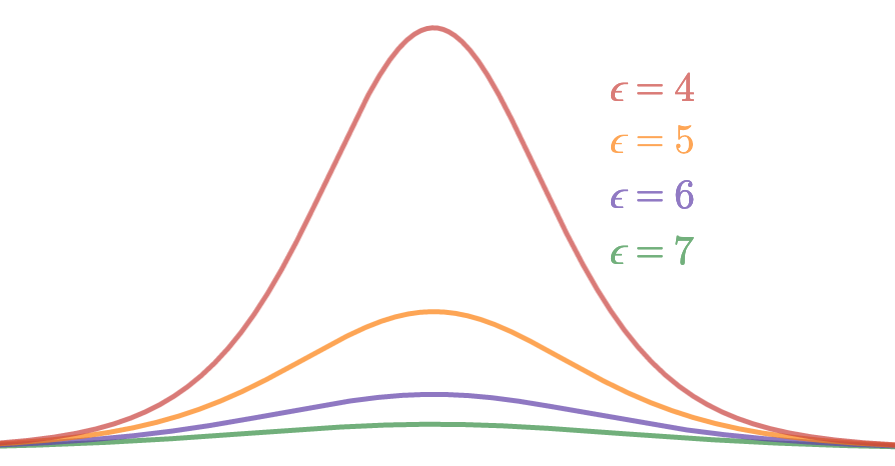
\includegraphics[width=0.7\linewidth]{img/regularizations.png}
  \caption{Force density functions using different amounts of regularization.}
  \label{fig:Regularization}
\end{figure}

We chose to implement these fundamental solutions for impulse and push response on a body. The force for an impulse is modeled as a regularized Dirac $\delta(t)$ function while the force for push is modeled as a Heaviside function $H(t)$.

\section{Method}

\subsection{Framework}

Our implementation \cite{Github} is written in C++ using the OpenFrameworks library \cite{OpenFrameworks}, a wrapper for OpenGL that provides mesh data structures. Starting from an initial mesh, we apply an impulse or push force to it at a given location using our \texttt{DisplacedMesh} class, which is responsible for simulating and displaying the result. It implements the solution to the linear elastodynamics equation in C++ for calculation on the CPU. Additionally, since the displacement for each vertex has no dependence on the displacement of any other vertex, the calculation is also implemented as a step in the vertex shader on the GPU. In both cases, it produces offsets for the original mesh vertices given their initial locations and the elapsed time. These offsetted vertices are then passed through the rest of the OpenGL pipeline to be rendered to the screen.

\subsection{Automatic Secondary Motion}

Given the ability to simulate the response of a mesh to a Kelvinlet force, we then need a way to generate these forces automatically from an input animation. Each frame, our system follows four steps:
\begin{itemize}
  \item For each vertex $X$ in the mesh, find its location $x$ for the current frame using the transformation $\phi(X)$ from the frame's bone positions.
  \item Approximate $\ddot{x}$ for all vertices using their locations from the past two frames of animation.
  \item Generate a Kelvinlet for each $x$ given its corresponding $\ddot{x}$a.
  \item Iteratively merge Kelvinlets that plausibly would have resulted from a single source impulse.
\end{itemize}
When generating initial per-vertex Kelvinlets, we refer to the definition of force $F = m\ddot{x}$ to obtain a direction and magnitude for the impulse force vector. We approximate that the user-provided mass of a mesh is evenly distributed across its vertices when picking a value for $m$. We pick a level of regularization $\epsilon$ such that there is a force of exactly $F$ at the location of the vertex:
$$\begin{aligned}
  \rho(0) &= F\\
  F \frac{15\epsilon^4}{8\pi(0^2 + \epsilon^2)^{7/2}} &= F\\
  \epsilon &= \left(\frac{15}{8\pi}-1\right)^{4/7}\\
  \epsilon &\approx 0.8\\
\end{aligned}$$

We then merge Kelvinlets. We only want to merge them if they are nearby and have near parallel force vectors. To check for closeness, we compute an approximate radius of the Kelvinlet's influence, only allowing Kelvinlets to merge if there is an intersection between the spheres produced by these radii. We pick the radius at which force magnitude drops to a low value (we use 0.1):
$$\begin{aligned}
  \left\Vert F\rho(r) \right\Vert &= 0.1\\
  \frac{15 \epsilon^4 \Vert F \Vert}{8\pi \left(r^2 + \epsilon^2\right)^{7/2}} &= 0.1\\
  r &= \sqrt{\left(\frac{15\epsilon^4 \Vert F \Vert}{0.1 \cdot 8\pi}\right)^{2/7} - \epsilon^2}
\end{aligned}$$

We additionally enforce Kelvinlet alignment by only allowing them to merge when $\hat{F}_1 \cdot \hat{F}_2 > 0.5$. If these conditions are met, then we compute the properties of the merged Kelvinlet. We aim to preserve the total amount of force, and since the space integral of regularized force varies only based on the scale of the force applied at the centre, this constrains the combined force magnitude. We make combined force direction a linear combination of the input force directions, weighted by the total amount of force in each. We use a similar linear combination to produce the new force centre $x'$. This gives us:
$$\begin{aligned}
  \Vert F' \Vert &= \Vert F_1 \Vert + \Vert F_2 \Vert\\
  \hat{F}' &= \frac{\Vert F_1 \Vert \hat{F}_1 + \Vert F_2 \Vert \hat{F}_2}{\Vert F_1 \Vert + \Vert F_2 \Vert}\\
  x' &= \frac{\Vert F_1 \Vert x_1 + \Vert F_2 \Vert x_2}{\Vert F_1 \Vert + \Vert F_2 \Vert}\\
\end{aligned}$$

Finally, we also need to pick a level of regularization $\epsilon'$ for the combined Kelvinlet. Ideally, it should regularize more the farther away the two force centers are, allowing the influence of the Kelvinlet to spread out and reach both. This leads us to the following formula, which augments a linear combination with a distance term:
$$\epsilon' = \frac{\Vert F_1 \Vert \epsilon_1 + \Vert F_2 \Vert \epsilon_2 + \min\{\Vert F_1\Vert, \, \Vert F_2 \Vert\} \Vert x_1 - x_2 \Vert}{\Vert F_1 \Vert + \Vert F_2 \Vert}$$

\section{Results}

\subsection{Stability}\label{Stability}

One of the benefits of Dynamic Kelvinlet based motion is that there is a closed-form solution for displacement, meaning there will not be any error accumulation or instability over time due to the integration scheme. However, within a single frame, there are still issues of stability due to numerical precision. This is largely due to the fact that some of the intermediate steps in calculating displacement include division by a factor of $r^3$. The paper includes a formula for the limit of displacement as $r \rightarrow 0$ to avoid division by 0 directly at the force application centre, but near the centre, if one uses the limit formula, it is equivalent to treating the whole neighbourhood around the centre as a rigid body. If one does not use the limit formula, one must deal with significant loss of precision. Using double precision floats and a single fourth-order Runge-Kutta (RK4) step, the paper treats a radius of 1e-4 around the centre as a rigid body. Since our implementation runs on graphics hardware in a shader, we are limited to single precision floats. We find that with a radius of 1e-2 and four RK4 steps, there is no noticeable precision error.


\begin{figure}[h]
  \centering
  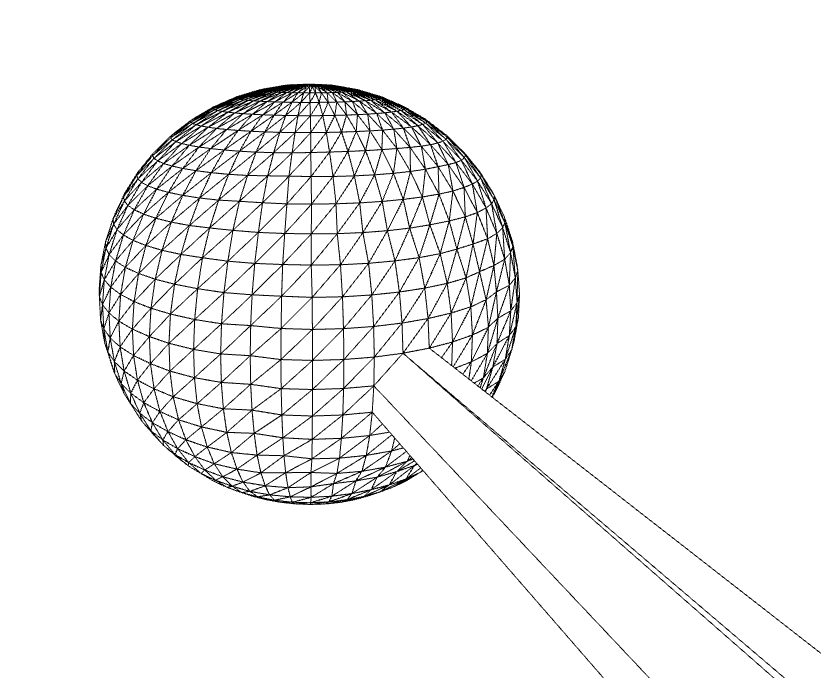
\includegraphics[width=0.7\linewidth]{img/precision-error-40.png}
  \caption{Catastrophic precision error around the impulse centre.}
  \label{fig:Catastrophic}
\end{figure}

\subsection{Performance}

Multiple versions of the Dynamic Kelvinlet system were implemented to assess how truly real-time it can be. As noted in Section \ref{Stability}, different implementations require different numbers of RK4 steps depending on the precision of the numbers used in the calculation. Profiling a CPU-based implementation using Linux's \texttt{perf} showed that most of the time was being taken by power function computations. Hence, a GPU-based version was also implemented. We only compare implementations without visual artifacts.

\begin{table}[h]
  \centering
  \begin{tabular}{lllr}
    Device & Precision & RK4 Steps & {\bf FPS} \\
    \hline
    CPU & double & 1 & {\bf 11.8} \\
    CPU & single & 4 & {\bf 3.8} \\
    GPU & single & 4 & {\bf 55.6} \\
  \end{tabular}
  \caption{Comparison of frame rates, in frames per second (FPS), of different Dynamic Kelvinlet implementations, with two Kelvinlets active.}
  \label{FrameRates}
\end{table}

Table \ref{FrameRates} shows the resulting frame rate when our different implementations are run on a late-2015 Macbook Pro. Our CPU-based implementations use a single core, and the GPU-based implementation uses the device's onboard Intel Iris Graphics 6100 chip. The reduced-size Stanford Dragon \cite{Stanford} mesh is used, which has 5205 vertices. Two Kelvinlet forces, one push and one impulse, are active on the mesh. The simulation frame rate is capped at 60 frames per second due to the limitations of the platform.

Even with 4 RK4 steps, the GPU-based implementation achieves significantly higher frame rates, nearly keeping up with the maximum platform refresh rate. This result supports the original paper's claim that the system can run in real time.

\subsection{Simulation Quality}

Although Dynamic Kelvinlets use physics to compute displacements over a field, real meshes are not infinite fields: they have boundaries and are not connected by an invisible, uniform continuum. To assess how plausible results look despite this assumption, we compare Kelvinlet forces applied to a continuum with a more traditional physics simulation of the application of a roughly equivalent force on a deformable body without this assumption.

We used the Bullet Physics \cite{Bullet} simulator packaged with Blender 2.8 \cite{Blender}. This models the mesh as a mass-spring system with springs along the edges of the mesh. A direct comparison with Dynamic Kelvinlets is not entirely possible because the two systems use different models. A single Dynamic Kelvinlet has a position, force, and amount of regularization; in Bullet, there is a force, position, and force field shape. The field shape defines the direction and magnitude of force for each point in space. Field shape options include vectors facing away from a point, vectors facing away from a line, vectors normal to a plane, and vectors pointing away from an arbitrary surface. The best analogue to a regularized Kelvinlet force in Bullet is a force field emanating from a point with an exponential distance falloff. For material properties, the Dynamic Kelvinlets system uses stiffness and compressibility; Bullet uses mass, spring stiffness, and friction. Once a force is created in Bullet, the material properties are manually tweaked to attempt to best match the Dynamic Kelvinlet response.

\begin{figure}[h]
  \centering
  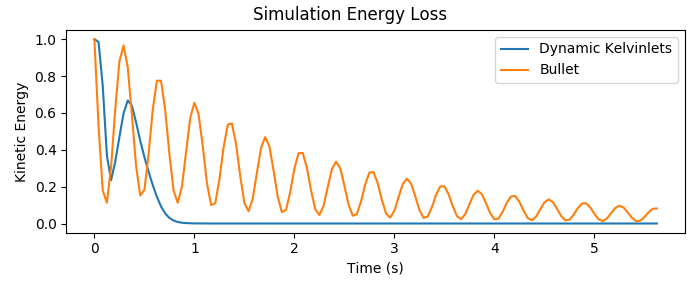
\includegraphics[width=\linewidth]{img/kinetic_energy.png}
  \caption{Kinetic energy over time present in the Dynamic Kelvinlet and Bullet simulations of the application of a single regularized impulse.}
  \label{fig:Energy}
\end{figure}

Immediately after the application of an impulse, the displacement in the neighbourhood of the impulse centre deforms similarly in the two systems. As time progresses, Bullet and Dynamic Kelvinlet responses diverge significantly. The most noticeable difference is that Bullet's mass-spring model continues to oscillate long after the impulse has been applied, whereas the Dynamic Kelvinlet response has a single pressure wave and a single shear wave. Figure \ref{fig:Energy} shows the kinetic energy over time for both simulations, communicating how the Bullet simulation continues moving for longer than the Dynamic Kelvinlet simulation. Note that since spring energy internal to the Bullet simulation is inaccessible when treated as a black box, only kinetic energy is shown rather than total energy of the system.

To assess the impact of the continuum assumption made by Dynamic Kelvinlets, we test on the Stanford Dragon \cite{Stanford} as a true wave would have to travel through its winding body rather than propagating directly outwards from the force centre as it would in a continuum with no gaps in space. While the continuum approximation produces inaccuracies on sharp, targeted forces, with large enough regularization of the impulse force, there is not much noticeable difference in displacement wave propagation between the continuum approximation and the mass-spring model. This is because the regularization spreads the force out enough that it has some influence across spatial gaps directly, without needing  to propagate through the volume of the mesh.

The response of force on soft bodies is usually perceived as a wave traveling through the body. Depending on the properties of the soft body, the dynamics might change, but the wave-like motion is well known. Spring-based models tend to give an oscillatory motion about the original location, which can differ from real life soft bodies when there are insufficient damping parameters. Dynamic Kelvinlets have an advantage over spring based methods for such cases, where erring on the side of having too few oscillations is preferable. This also results in more easily controllable responses, as the influence of a single force has a tighter bound in time, which can be preferable for artists and animators.

Another point of note is that the input to Dynamic Kelvinlets includes the material properties of the soft body rather than the mass and the spring constants. Not only does that make the setup of the simulation faster, it also makes it more intuitive as it is easier to identify material properties than to identify the spring constants for an object.

A final note is that the Bullet simulation ran at around 19 frames per second on the CPU. This type of simulation has the capability of achieving decent performance, but its ability to parallelize further is limited due to information dependencies in steps of the simulation algorithm.

\subsection{Secondary Motion Quality}

TODO

\section{Future Work}

TODO

%%
%% The next two lines define the bibliography style to be used, and
%% the bibliography file.
\bibliographystyle{ACM-Reference-Format}
\bibliography{report}

\end{document}
\endinput
%%
